\section{Consuntivazione}

\subsection{Milestones:}
\begin{itemize}
    \item Release versione 0.0.4 dell'analisi dei requisiti (Completa al: 100\%)
    \item Release versione 0.0.5 dell'analisi dei requisiti (Completa al: 60\%)
\end{itemize}

\subsection{Attività svolte}

\begin{table}[H]
    \begin{xltabular}{\textwidth}{X l l}
        
        \rowcolor{gray!30} \textbf{Attività} & \textbf{Stato} & \textbf{Ruolo}\\
        \endhead
        \hline
        riviste e riorganizzate tutte le uc & completato & Analista \\
        rilasciata versione 0.0.4 dell'analisi dei requisiti & completato & Responsabile \\
        finalizzata documentazione del \textbf{PoC} & completato & Analista \\
        normata codifica dei requisiti & parziale & Amministratore \\
    \end{xltabular}
    \caption{Lista delle attività svolte durante lo sprint}
\end{table}


\begin{table}[ht]
    \begin{tabularx}{\linewidth}{X|rrrrrrr}
    \rowcolor{gray!30}& Re & Amm & An & Pro & Prog & Ver & tot \\
    \hline
    Bonavigo Michele                        & 0,5 & 0 & 0 & 0 & 0 & 0  & 0,5 \\
    \rowcolor{gray!10}Casarotto Mattia      & 0 & 0 & 0 & 0 & 0 & 0 & 0 \\
    Massarenti Alessandro                   & 0,7 & 0 & 0 & 0 & 0 & 0,4  & 1,1 \\
    \rowcolor{gray!10}Peron Samuel          & 0 & 0 & 0 & 0 & 0 & 0 & 0 \\
    Pierobon Luca                           & 0 & 0 & 0,75 & 0 & 0 & 0,35 & 1,1 \\
    \rowcolor{gray!10}Romano Davide         & 0 & 0 & 0 & 0 & 0 & 0 & 0 \\
    Zarantonello Giorgio                    & 0 & 0 & 0 & 0 & 0 & 0 & 0 \\
    \hline                                  & 1,2 & 0 & 0,75 & 0 & 0 & 0,75 & \\
    \end{tabularx}
    \caption{\label{ruoli-persone}Spartizione dei ruoli e ore svolte durante lo sprint}
\end{table}

\begin{center}
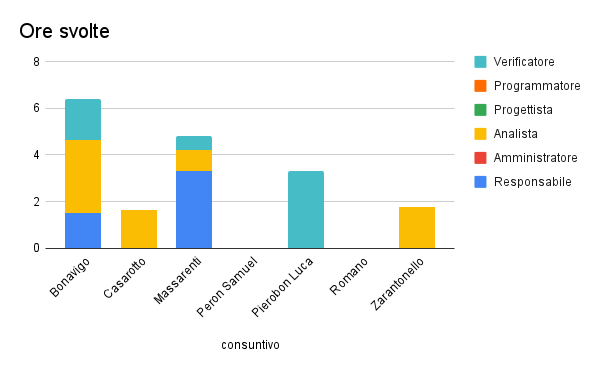
\includegraphics[width=12cm]{img/ore-svolte.png}
\end{center}

\begin{table}[ht]
    \begin{tabularx}{\linewidth}{X|l|l}
    \rowcolor{gray!30}& Ore & Costo \\
    \hline
    
    Responsabile & 1,2 & € 36,00 \\
    \rowcolor{gray!10}Amministratore & 0 & € 0,00 \\
    Analista & 0,75 & € 18,75 \\
    \rowcolor{gray!10}Progettista & 0 & € 0,00 \\
    Programmatore & 0 & € 0,00 \\
    \rowcolor{gray!10}Verificatore & 0,75 &€ 11,25 \\
    totale & 2,7 & € 66,00 \\
    \end{tabularx}
    \caption{\label{costi-ruolo}Spartizione dei ruoli e ore svolte durante lo sprint}
\end{table}

Avendo quindi consumato €66,00\footnote{Si veda tabella \ref{costi-ruolo}} del budget durante questo sprint, rimangono ancora a disposizione € 11306,50 per gli sprint seguenti.

\subsection{Trend e riflessioni}\label{subsec:trend}

\begin{figure}[H]
    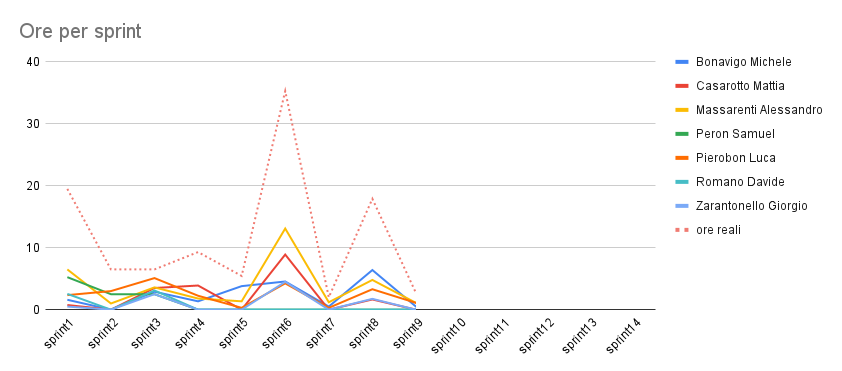
\includegraphics[width=\linewidth]{img/andamento.png}
    \caption{Andamento ore utilizzate nei vari sprint}\label{img:andamento}
\end{figure}

Durante questo sprint, purtroppo, l'attività degli esami si è intensificata per tutti i membri del gruppo. Nonostante i buoni propositi prefissati, le attività di progetto sono drasticamente rallentate.

Prevediamo nel prossimo sprint di recuperare il tempo perduto.

\subsection{Difficoltà e problemi di sprint}

Non ci sono state grandi difficoltà esterne durante questo sprint. Purtroppo però, come negli sprint appena precedenti, non siamo ancora riusciti a definire con il proponente il supporto hardware per i lampioni a cui dovremo fare fede.

Internamente, come difficoltà, si rimanda alla riflessione posta nella sezione \ref{subsec:trend}.

Queste verranno discusse in sede di preparazione del prossimo sprint.
